\section{空間與位置分配}

\begin{frame}{source code}
    \begin{columns}[t]
        \column{.45\textwidth}
        \begin{adjustbox}{keepaspectratio}
            \lstinputlisting{../a.c}
        \end{adjustbox}
        \column{.45\textwidth}
        \begin{adjustbox}{keepaspectratio}
            \lstinputlisting{../b.c}
        \end{adjustbox}
    \end{columns}
\end{frame}

\begin{frame}{合併目的檔}
    \begin{itemize}
        \item 按序累加(圖4-1)
        \item 相似區段合併(圖4-2)
    \end{itemize}
\end{frame}


\begin{frame}{按序累加}
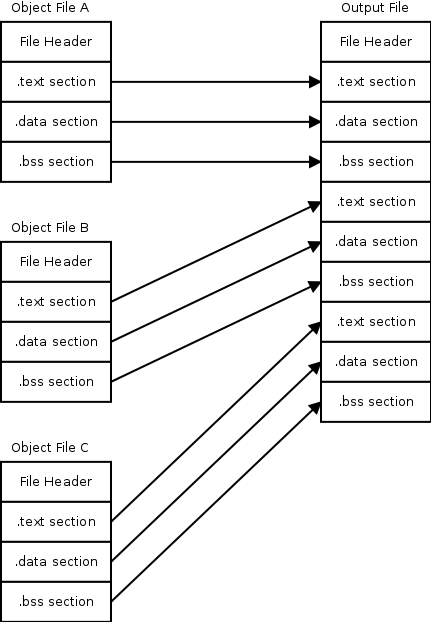
\includegraphics[height=.8\textheight]{./img/4-1.png}
\end{frame}

\begin{frame}{相似區段合併}
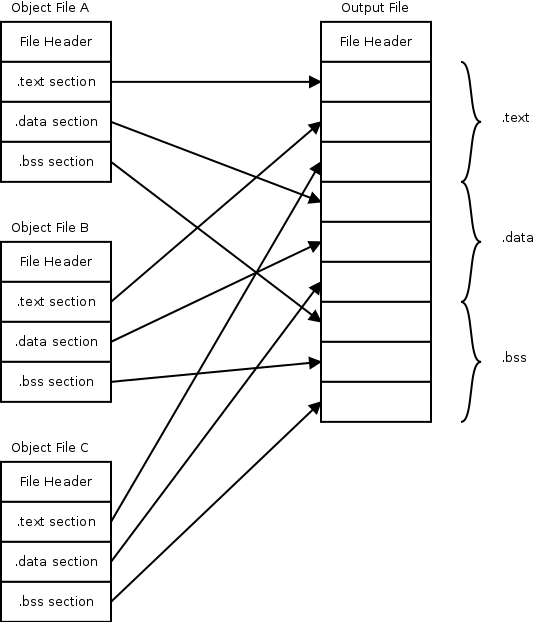
\includegraphics[height=.8\textheight]{./img/4-2.png}
\end{frame}



\begin{frame}{相似區段合併}
    \begin{itemize}
        \item Step1 空間與位置分配\footnote[1]{在Linux 下, ELF 可執行檔預設從位置0x08048000開始分配}
        \item Step2 符號解析與重定
    \end{itemize}
\end{frame}


\section{符號解析與重定}

\begin{frame}
    \$ gcc -c a.c\\
    \$ objdump -d a.o
    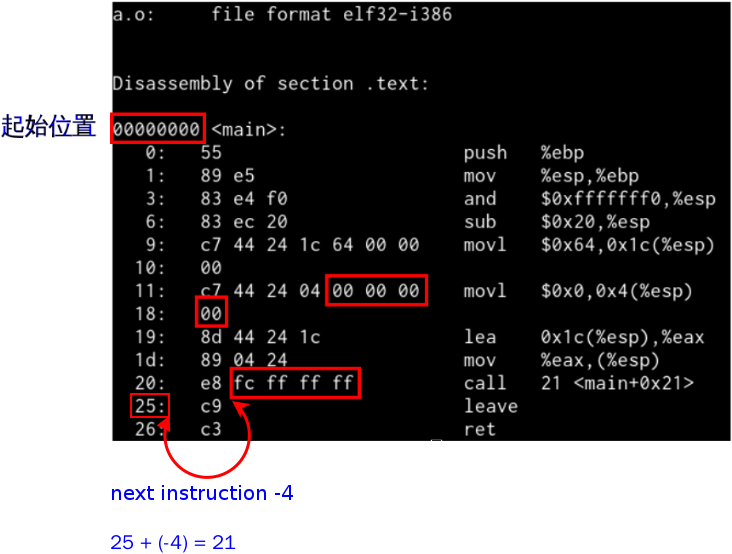
\includegraphics[height=.8\textheight]{./img/objdump-ao1.png}
    %\includegraphics[width=\textwidth]{./img/objdump-d-a.o.png}
\end{frame}

\begin{frame}{mechine code format}
    \begin{itemize}
        \item mov指令
        \begin{itemize}
            \item offset address: 0x11
            \item opcode: C4 44 24 04 (mov)
            \item 'shared': 00 00 00 00
        \end{itemize}
        \item 相對偏移呼叫指令call
        \begin{itemize}
            \item offset address: 0x20
            \item opcode: E8 (call)
            \item 'swap': FC FF FF FF\footnote[2]{目標位置相對於下一個指令的offset}
        \end{itemize}
    \end{itemize}
\end{frame}

\begin{frame}{連結後的輸出程式'ab'反組譯}
    \$ ld a.o b.o -e main -o ab\\
    \$ objdump -d ab\\
    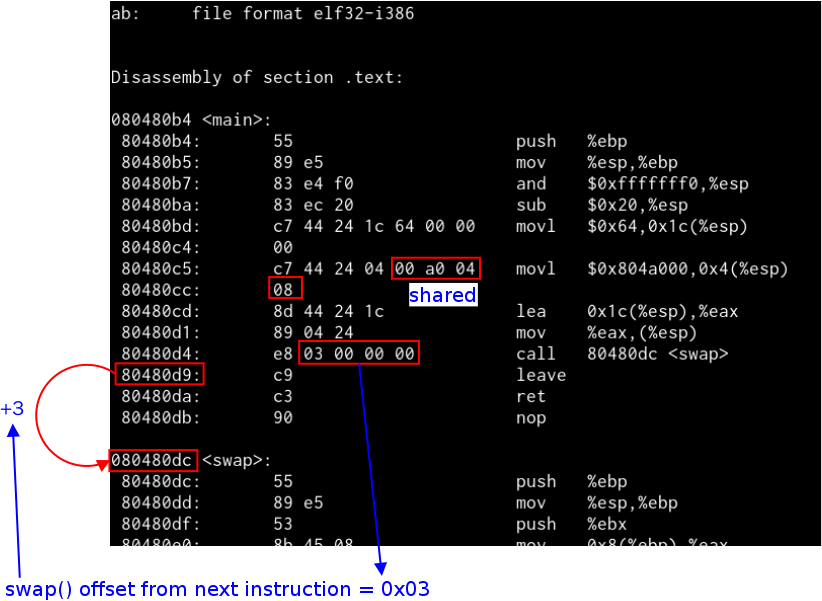
\includegraphics[height=.7\textheight]{./img/objdump-ab1.png}
    %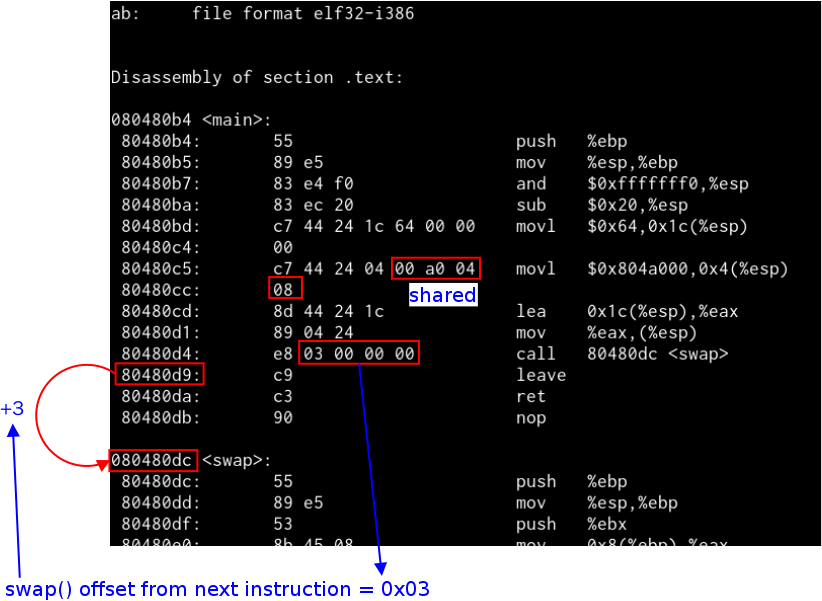
\includegraphics[width=\textwidth]{./img/objdump-ab1.png}
\end{frame}

\begin{frame}{重定表}
    \$ objdump -d a.o\\
    \$ ld a.o \#(error)\\
    \$ objdump -r a.o
    %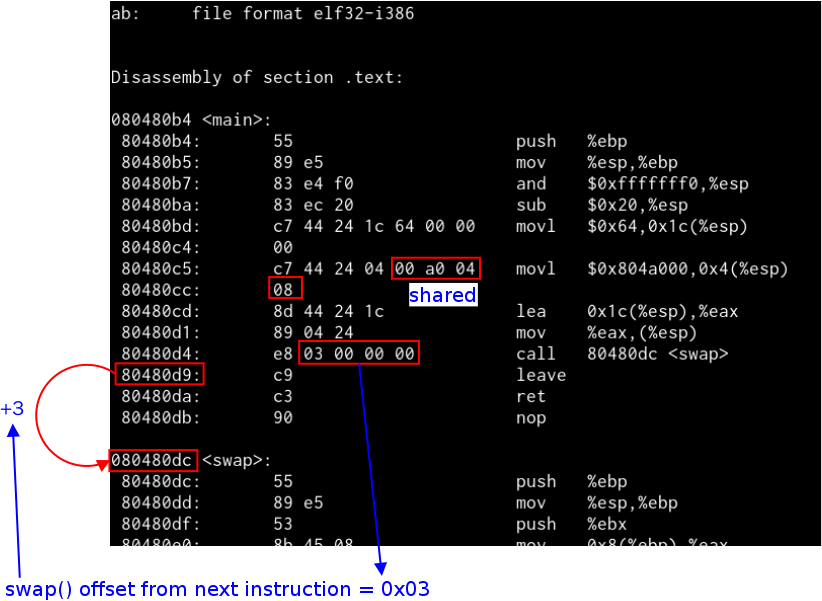
\includegraphics[height=.8\textheight]{./img/objdump-ab1.png}
    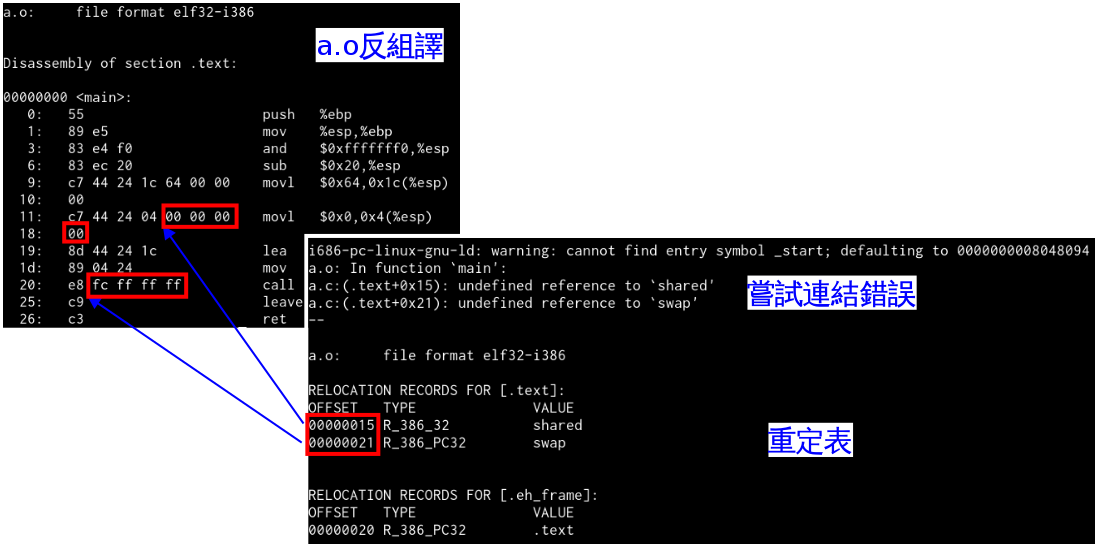
\includegraphics[width=\textwidth]{./img/relocationtbl1.png}
\end{frame}

\begin{frame}{符號解析}
    \$ readelf -s a.o
    %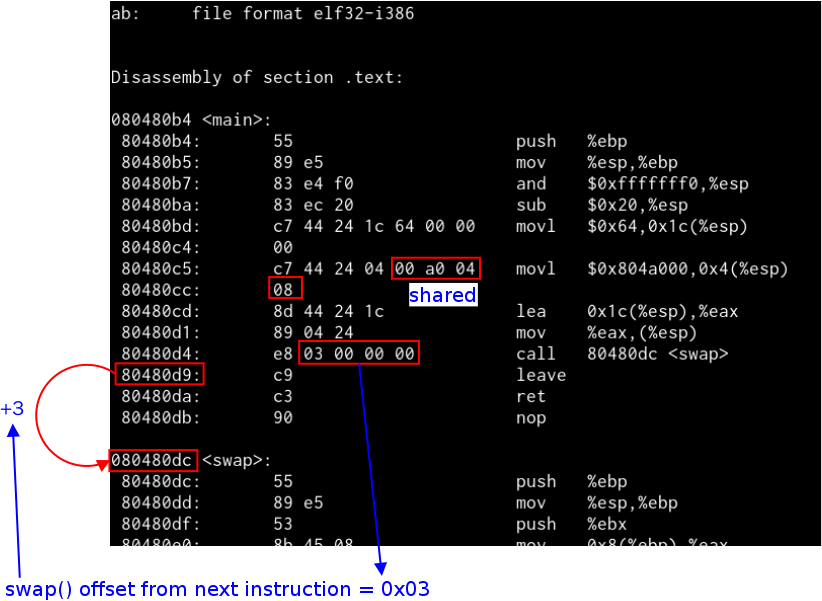
\includegraphics[height=.8\textheight]{./img/objdump-ab1.png}
    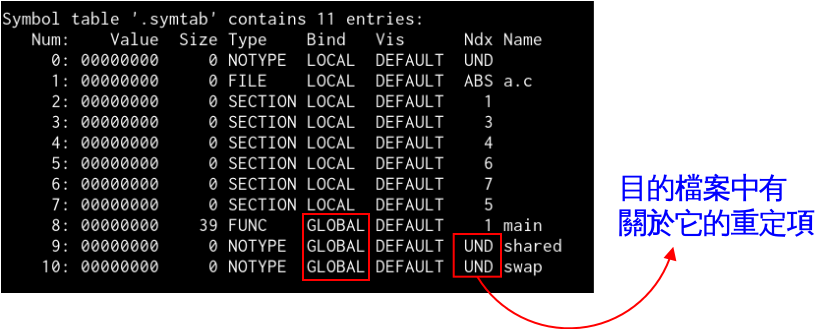
\includegraphics[width=\textwidth]{./img/readelf-s-ao1.png}
\end{frame}


\begin{frame}{指令修正方式}
    \begin{itemize}
        \item 絕對近址32位定址\\
            R\_386\_32 = S + A
        \item 相對近址32位定址\\
            R\_386\_PC32 = S + A - P
        \item 
        \begin{itemize}
            \item S: 符號的實際位置
            \item A: 保存在被修正位置的值
            \item P: 相對於區段開始的偏移量
        \end{itemize}
    \end{itemize}
\end{frame}


\begin{frame}{example}
    \begin{itemize}
        \item main(): VA at 0x1000
        \item swap(): VA at 0x2000
        \item shared: VA at 0x3000
        \item relocation table:
            \begin{itemize}
                \item shared: R\_386\_32\\
                   S + A = 0x3000 + 0x00 = 0x3000
                \item swap: R\_386\_PC32\\
                   P = 0x1000 + 0x21 = 0x1021\\
                   S + A - P = 0x2000 + (-4) - 0x1021 = 0x0fdb
            \end{itemize}
    \end{itemize}
\end{frame}

\section{COMMON區塊}

\begin{frame}{Alignment}
    \begin{itemize}
        \item 強符號個數大於2\\
            illegle
        \item 強符號*1, 弱符號*N\\
            以強符號為準\\
            (如果弱符號的大小,大於強符號,linker會有警告:\\
            ld: warning: alignment 4 of symbol "global" in a.o is smaller
            than 8 in b.o)
        \item 弱符號*N\\
            選大小最大的
    \end{itemize}
\end{frame}


\begin{frame}{COMMON to BSS}
    \begin{itemize}
        \item 未初始化的全域變數放進: COMMON
        \item 涉及強弱符號,linking 的時候確認之後放進: BSS
        \item 總體來看,還是放在BSS
        \item GCC 參數設定不允許放COMMON:\\
            "-fno-common"
    \end{itemize}
\end{frame}

\begin{frame}{smallest program}{inline assembly/linker script}
    \begin{columns}[t]
        \column{.4\textwidth}
        Inline Assembly
        \begin{figure}
            \begin{center}
                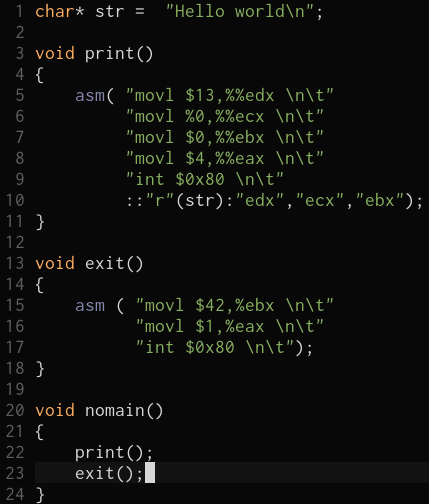
\includegraphics[width=\textwidth]{./img/inlineasm.png}
                \caption{TinyHelloWorld.c}
            \end{center}
        \end{figure}
        \column{.5\textwidth}
        Linker Script
         \begin{figure}
            \begin{center}
                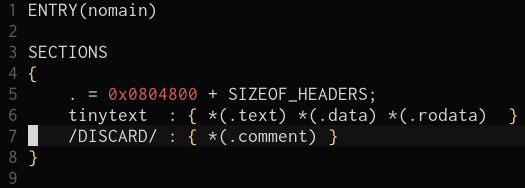
\includegraphics[width=\textwidth]{./img/linkscript.png}
                \caption{TinyHelloWorld.lds}
            \end{center}
        \end{figure}
    \end{columns}
\end{frame}
